\documentclass[10pt, a4paper]{article}
\usepackage[utf8]{inputenc}
\usepackage[T1]{fontenc}
\usepackage[spanish, es-tabla, es-nodecimaldot]{babel}
\usepackage{geometry}
\geometry{top=1.6cm, bottom=1.6cm, left=1.4cm, right=1.4cm}
\usepackage{amsmath, amssymb}
\usepackage{booktabs}
\usepackage{array}
\usepackage{tabularx}
\usepackage{multirow}
\usepackage{graphicx}
\usepackage{caption}
\usepackage{xcolor}
\usepackage{fancyhdr}
\usepackage{enumitem}
\usepackage{float}
\usepackage{colortbl}
\usepackage{tcolorbox}
\usepackage{tikz}
\usetikzlibrary{shapes,arrows.meta,positioning,calc,fit,backgrounds}
\usepackage[siunitx, RPvoltages, americanresistors]{circuitikz}
\sisetup{output-decimal-marker = {,}}

% Colores institucionales y técnicos
\definecolor{utnblue}{RGB}{18, 65, 130}
\definecolor{darkred}{RGB}{180, 20, 20}
\definecolor{darkgreen}{RGB}{20, 130, 40}
\definecolor{softgray}{RGB}{247, 249, 252}
\definecolor{railpos}{RGB}{220, 50, 50}
\definecolor{railneg}{RGB}{50, 100, 220}
\definecolor{railgnd}{RGB}{60, 60, 60}

\usepackage[plainpages=false, pdfpagelabels=true]{hyperref}
\hypersetup{
    colorlinks=true,
    linkcolor=utnblue,
    urlcolor=utnblue,
    citecolor=utnblue,
    pdfencoding=auto,
    psdextra
}

\pagestyle{fancy}
\fancyhf{}
\lhead{\small \textbf{Electrónica Aplicada II} --- UTN FRC (2026)}
\rhead{\small \textbf{TP N.º 2}: Guía Visual de Montaje en Protoboard (TL084)}
\cfoot{\small Página \thepage}
\renewcommand{\headrulewidth}{0.5pt}

\newtcolorbox{alerta}[1][]{
    colback=red!5!white,
    colframe=red!75!black,
    fonttitle=\bfseries,
    title=#1,
    arc=2pt,
    boxrule=0.8pt,
    left=6pt, right=6pt, top=4pt, bottom=4pt
}

\newtcolorbox{notabox}[1][]{
    colback=softgray,
    colframe=utnblue!70!black,
    fonttitle=\bfseries,
    title=#1,
    arc=2pt,
    boxrule=0.8pt,
    left=6pt, right=6pt, top=4pt, bottom=4pt
}

\begin{document}

% ==================== PÁGINA 1: ENCABEZADO, INTRODUCCIÓN Y PINOUT ====================
\begin{center}
    {\large \textsc{\textbf{Universidad Tecnológica Nacional --- Facultad Regional Córdoba}}}\\[2pt]
    {\normalsize Departamento de Ingeniería Electrónica --- Cátedra de Electrónica Aplicada II}\\[4pt]
    {\LARGE \bfseries \color{utnblue} Guía Visual Literal de Montaje en Protoboard}\\[2pt]
    {\Large \bfseries Diagramas Gráficos y Tablas de Coordenadas Orificio por Orificio}\\[3pt]
    {\small \textbf{Trabajo Práctico de Laboratorio N.º 2} \quad---\quad \textbf{3 $\times$ TL084 (DIP-14), Valores 100\% Normalizados}}
\end{center}
\vspace{-6pt}
\noindent\rule{\textwidth}{1pt}
\vspace{2pt}

\section{Introducción y Mapeo del Sistema}

Esta guía técnica proporciona el \textbf{esquema gráfico visual literal de conexionado en protoboard} para armar desde cero el circuito completo del TP N.º~2. Incluye para cada etapa:
\begin{enumerate}[itemsep=1pt, topsep=1pt]
    \item El diagrama gráfico a escala de la protoboard indicando los orificios exactos donde se inserta cada pata de cada componente.
    \item La tabla de coordenadas físicas (fila 1 a 30, columnas A a J, rieles de alimentación) para verificar cada cable y componente individualmente.
\end{enumerate}

El sistema toma como entrada una onda cuadrada de $f = \SI{4300}{\hertz}$ ($0\text{ a }+2.5\text{ V}$) provista por el generador de funciones y genera sucesivamente:
\begin{itemize}[itemsep=1pt, topsep=1pt]
    \item \textbf{Señal 1}: Onda cuadrada adaptada a una impedancia de entrada normalizada de \textbf{$\SI{15}{\kilo\ohm}$}.
    \item \textbf{Señal 2}: Onda triangular de \textbf{$\SI{-1.5}{\volt}$ a $\SI{+4.0}{\volt}$} ($V_{pp} = \SI{5.5}{\volt}$, continua $+1.25\text{ V}$).
    \item \textbf{Señal 3}: Onda cuadrada de \textbf{$\SI{0.0}{\volt}$ a $\SI{+3.0}{\volt}$} ($V_{pp} = \SI{3.0}{\volt}$, continua $+1.5\text{ V}$).
    \item \textbf{Señal 4}: Tren de pulsos rectificados positivos de \textbf{$\SI{0.0}{\volt}$ a $\SI{+1.0}{\volt}$}, generados en cada flanco de Señal 3.
\end{itemize}

\section{Pinout Oficial del Integrado Cuádruple TL084 (DIP-14)}

\begin{figure}[H]
\centering
\begin{tikzpicture}[scale=0.82, every node/.style={font=\footnotesize}]
  \fill[softgray] (0,0) rectangle (4,7);
  \draw[thick, draw=black!80, rounded corners=3pt] (0,0) rectangle (4,7);
  \draw[thick, fill=white] (1.6,7) arc (0:-180:0.4);
  \node at (2,6.4) {\bfseries \large TL084};
  \node at (2,5.9) {\color{utnblue}\bfseries DIP-14 (Vista Superior)};
  
  \foreach \p/\y/\lbl/\col in {%
    1/6.5/{OUT 1 (OpAmp A)}/{darkgreen},%
    2/5.5/{IN- 1 (OpAmp A)}/{darkgreen},%
    3/4.5/{IN+ 1 (OpAmp A)}/{darkgreen},%
    4/3.5/{+12V ($V_{CC}^+$)}/{railpos},%
    5/2.5/{IN+ 2 (OpAmp B)}/{utnblue},%
    6/1.5/{IN- 2 (OpAmp B)}/{utnblue},%
    7/0.5/{OUT 2 (OpAmp B)}/{utnblue}%
  } {%
    \fill[black!30] (-0.5,\y-0.12) rectangle (0,\y+0.12);
    \draw[thick] (-0.5,\y) -- (0,\y);
    \node[left, text=\col] at (-0.5,\y) {\bfseries \lbl};
    \node[right, text=black] at (0.05,\y) {\bfseries \p};
  }
  
  \foreach \p/\y/\lbl/\col in {%
    14/6.5/{OUT 4 (OpAmp D)}/{darkred},%
    13/5.5/{IN- 4 (OpAmp D)}/{darkred},%
    12/4.5/{IN+ 4 (OpAmp D)}/{darkred},%
    11/3.5/{-12V ($V_{EE}^-$)}/{railneg},%
    10/2.5/{IN+ 3 (OpAmp C)}/{purple!80!black},%
    9/1.5/{IN- 3 (OpAmp C)}/{purple!80!black},%
    8/0.5/{OUT 3 (OpAmp C)}/{purple!80!black}%
  } {%
    \fill[black!30] (4,\y-0.12) rectangle (4.5,\y+0.12);
    \draw[thick] (4,\y) -- (4.5,\y);
    \node[right, text=\col] at (4.5,\y) {\bfseries \lbl};
    \node[left, text=black] at (3.95,\y) {\bfseries \p};
  }
\end{tikzpicture}
\caption{Distribución física de pines del TL084 (DIP-14).}
\label{fig:pinout_tl084}
\end{figure}

\begin{alerta}[¡ADVERTENCIA CRÍTICA DE ALIMENTACIÓN RESPECTO AL TL082!]
En el integrado doble TL082 (DIP-8), $+V_{CC}$ es el Pin 8 y $-V_{EE}$ es el Pin 4.\\
En el \textbf{TL084 (DIP-14)}, la alimentación es:
\textbf{Pin 4 $\to +12\text{ V}$} y \textbf{Pin 11 $\to -12\text{ V}$}.\\
\textbf{Invertir esta conexión o aplicar $-12\text{ V}$ en el pin 4 destruirá de inmediato el integrado.}
\end{alerta}

\newpage

% ==================== PÁGINA 2: VISTA PANORÁMICA Y ESTRATEGIA ====================
\section{Estrategia de Montaje y Vista Panorámica General}

El circuito se divide de forma limpia y modular en \textbf{3 protoboards estándar}:
\begin{itemize}[itemsep=2pt, topsep=1pt]
    \item \textbf{Protoboard 1 ($U_1$)}: Entrada $Z_i = \SI{15}{\kilo\ohm}$ (Señal 1), acondicionamiento de Offset, Integrador Miller y Centrador de \textbf{Señal 2} ($\SI{-1.5}{\volt}$ a $\SI{+4.0}{\volt}$).
    \item \textbf{Protoboard 2 ($U_2$)}: Derivador Miller compensado, conformador de continua de \textbf{Señal 3} ($\SI{0}{\volt}$ a $\SI{+3.0}{\volt}$), inversor conformador y rectificador Rama A.
    \item \textbf{Protoboard 3 ($U_3$)}: Rectificador Rama B, sumador y amplificador de pulsos de \textbf{Señal 4} ($\SI{0}{\volt}$ a $\SI{+1.0}{\volt}$) y terminación segura de operacionales libres.
\end{itemize}

\begin{figure}[H]
\centering
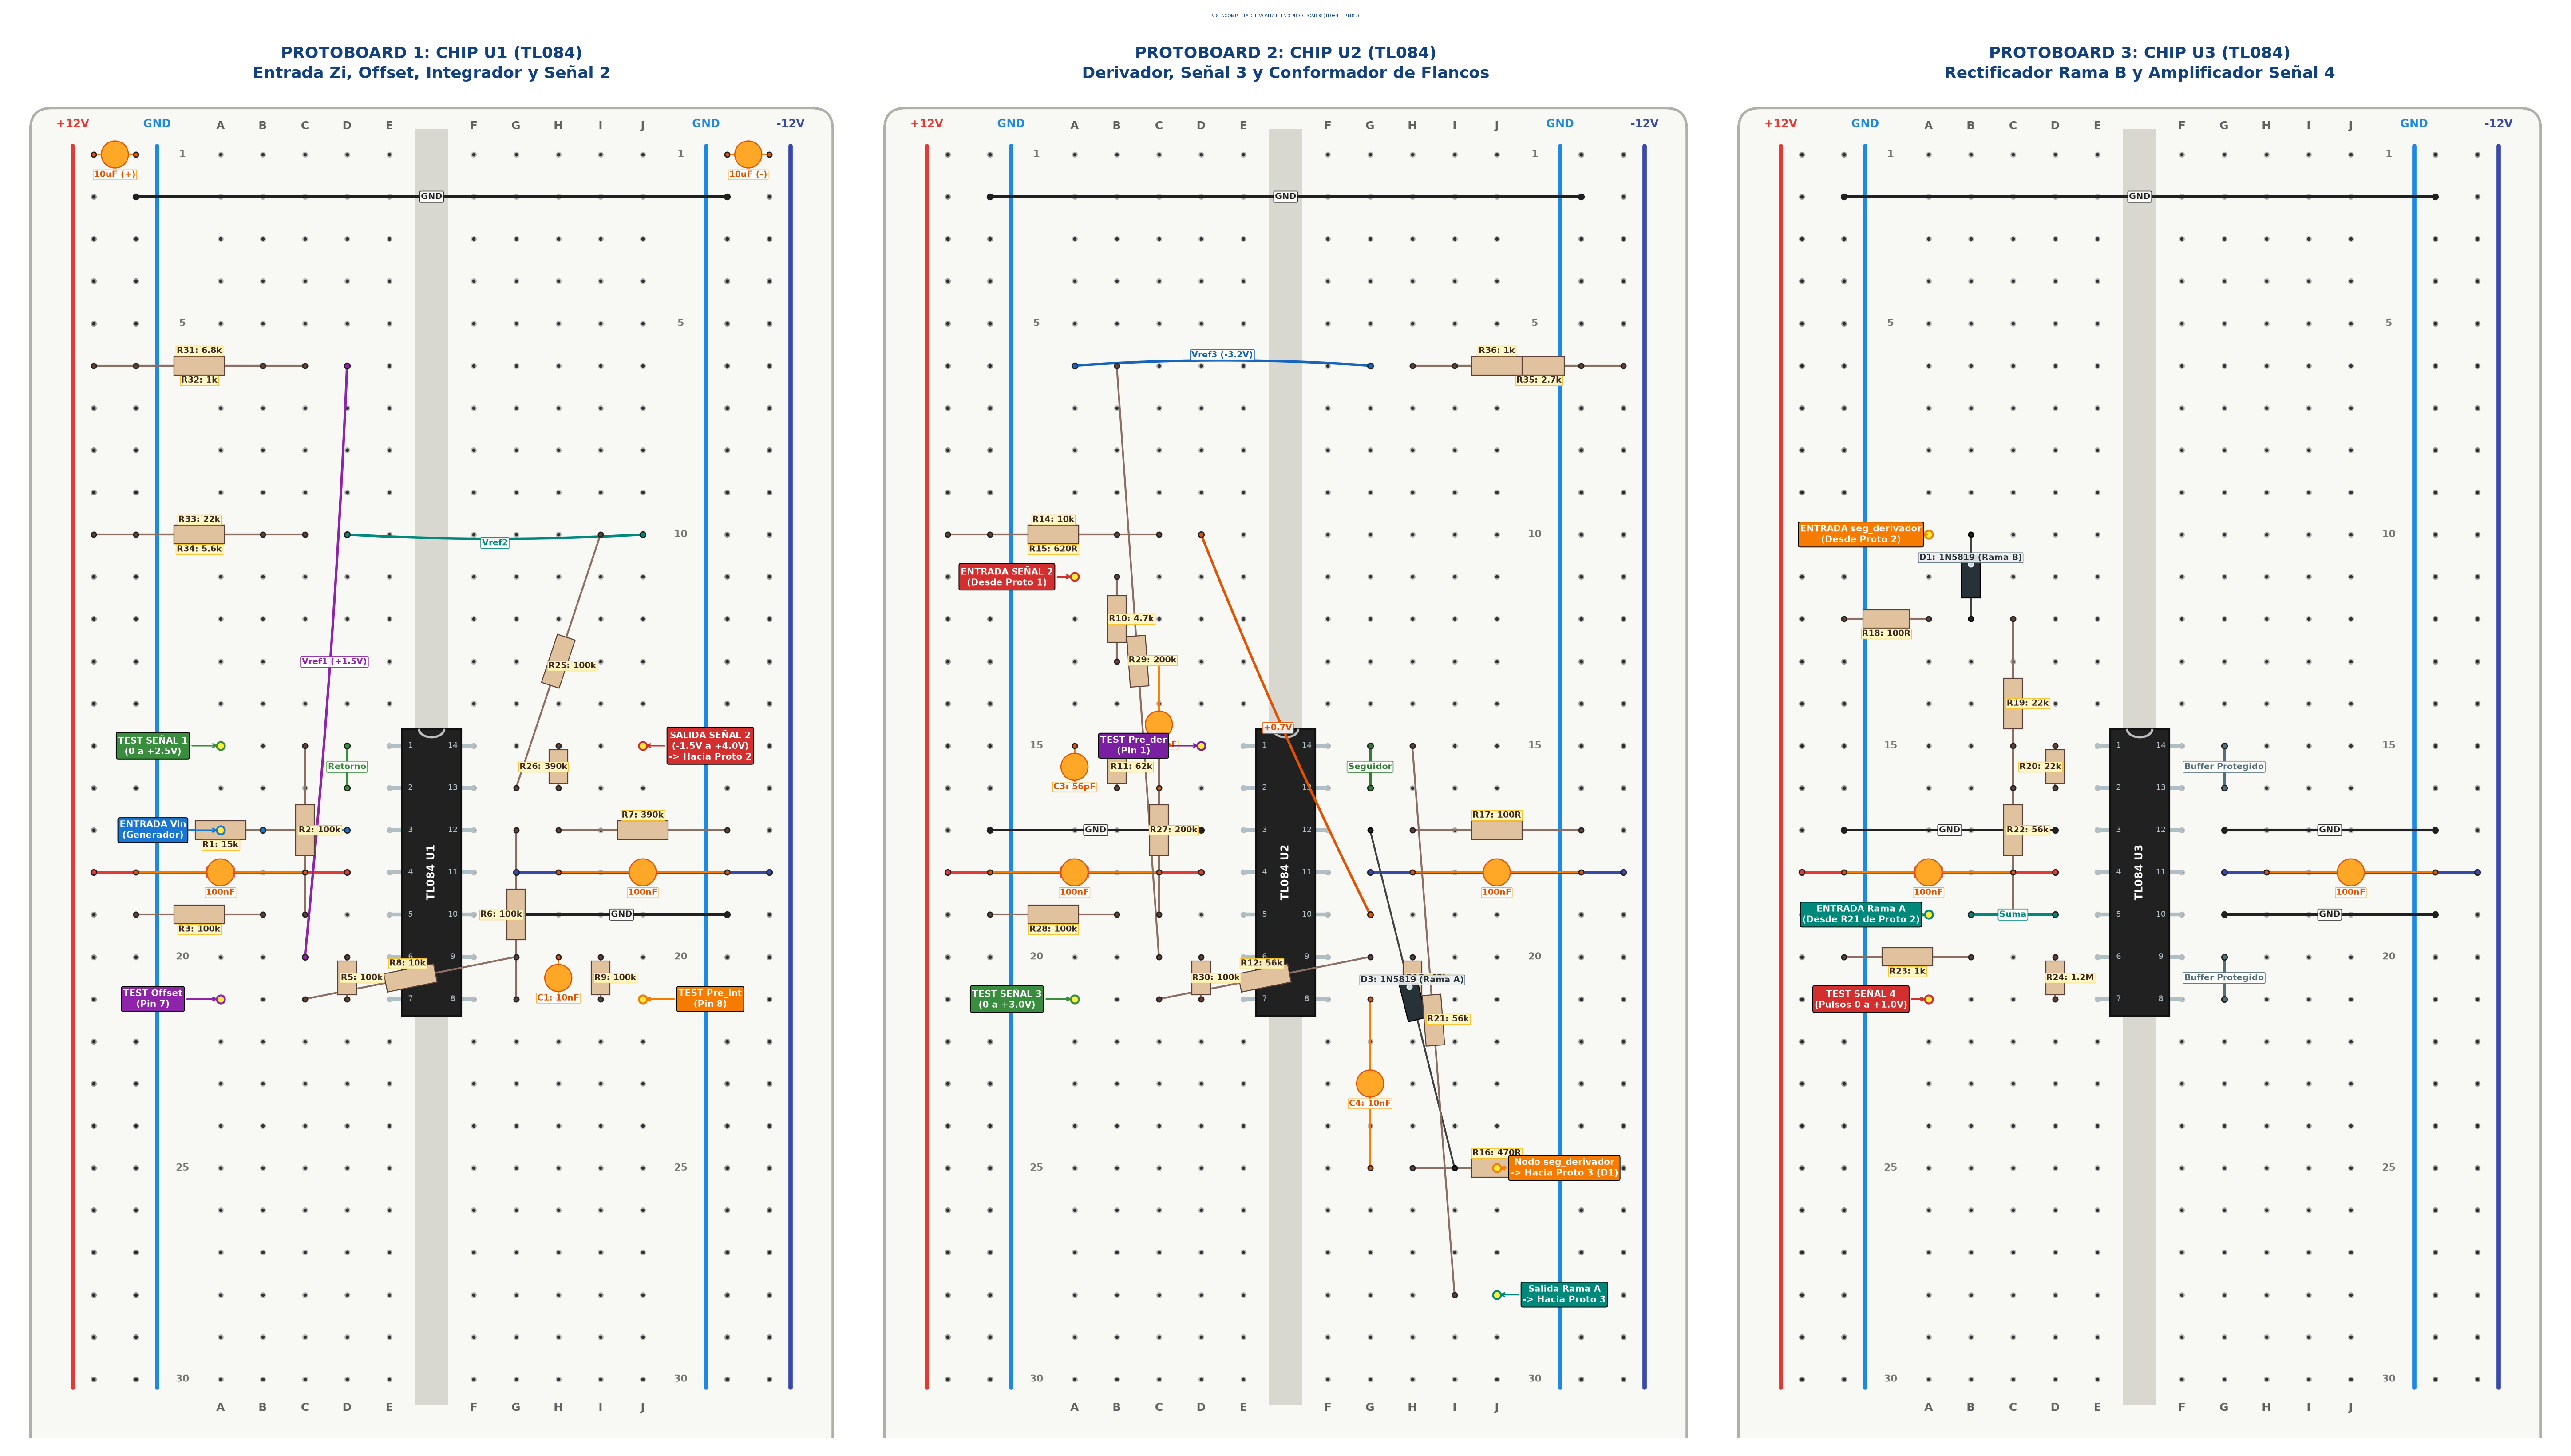
\includegraphics[width=\textwidth]{simulacion/protoboard_completa.png}
\caption{Vista panorámica del montaje en 3 protoboards con sus respectivos circuitos integrados TL084.}
\label{fig:proto_completa}
\end{figure}

\subsection{Reglas de Conexión de Rieles de Alimentación y Desacoplo}
\begin{itemize}[itemsep=2pt, topsep=1pt]
    \item \textbf{Rieles Izquierdos}: Exterior = \textbf{$+12\text{ V}$} (rojo), Interior = \textbf{GND} (azul).
    \item \textbf{Rieles Derechos}: Interior = \textbf{GND} (azul), Exterior = \textbf{$-12\text{ V}$} (azul oscuro/violeta).
    \item \textbf{Puentes de Masa}: Unir con jumper negro los rieles de masa izquierdo y derecho en la fila 2 de cada protoboard.
    \item \textbf{Desacoplo de Alta Frecuencia}: Capacitor cerámico de $\SI{100}{\nano\farad}$ (104) directo entre Pin 4 ($+12\text{ V}$) y GND, y entre Pin 11 ($-12\text{ V}$) y GND en cada uno de los 3 chips.
    \item \textbf{Filtrado Bulk}: Dos electrolíticos de $\SI{10}{\micro\farad} / \SI{25}{\volt}$ en la fila 1 de la entrada general.
\end{itemize}

\newpage

% ==================== PÁGINA 3: PROTOBOARD 1 (DIAGRAMA) ====================
\section{Protoboard 1: Esquema Gráfico Literal (Chip \texorpdfstring{$U_1$}{U1})}

\begin{center}
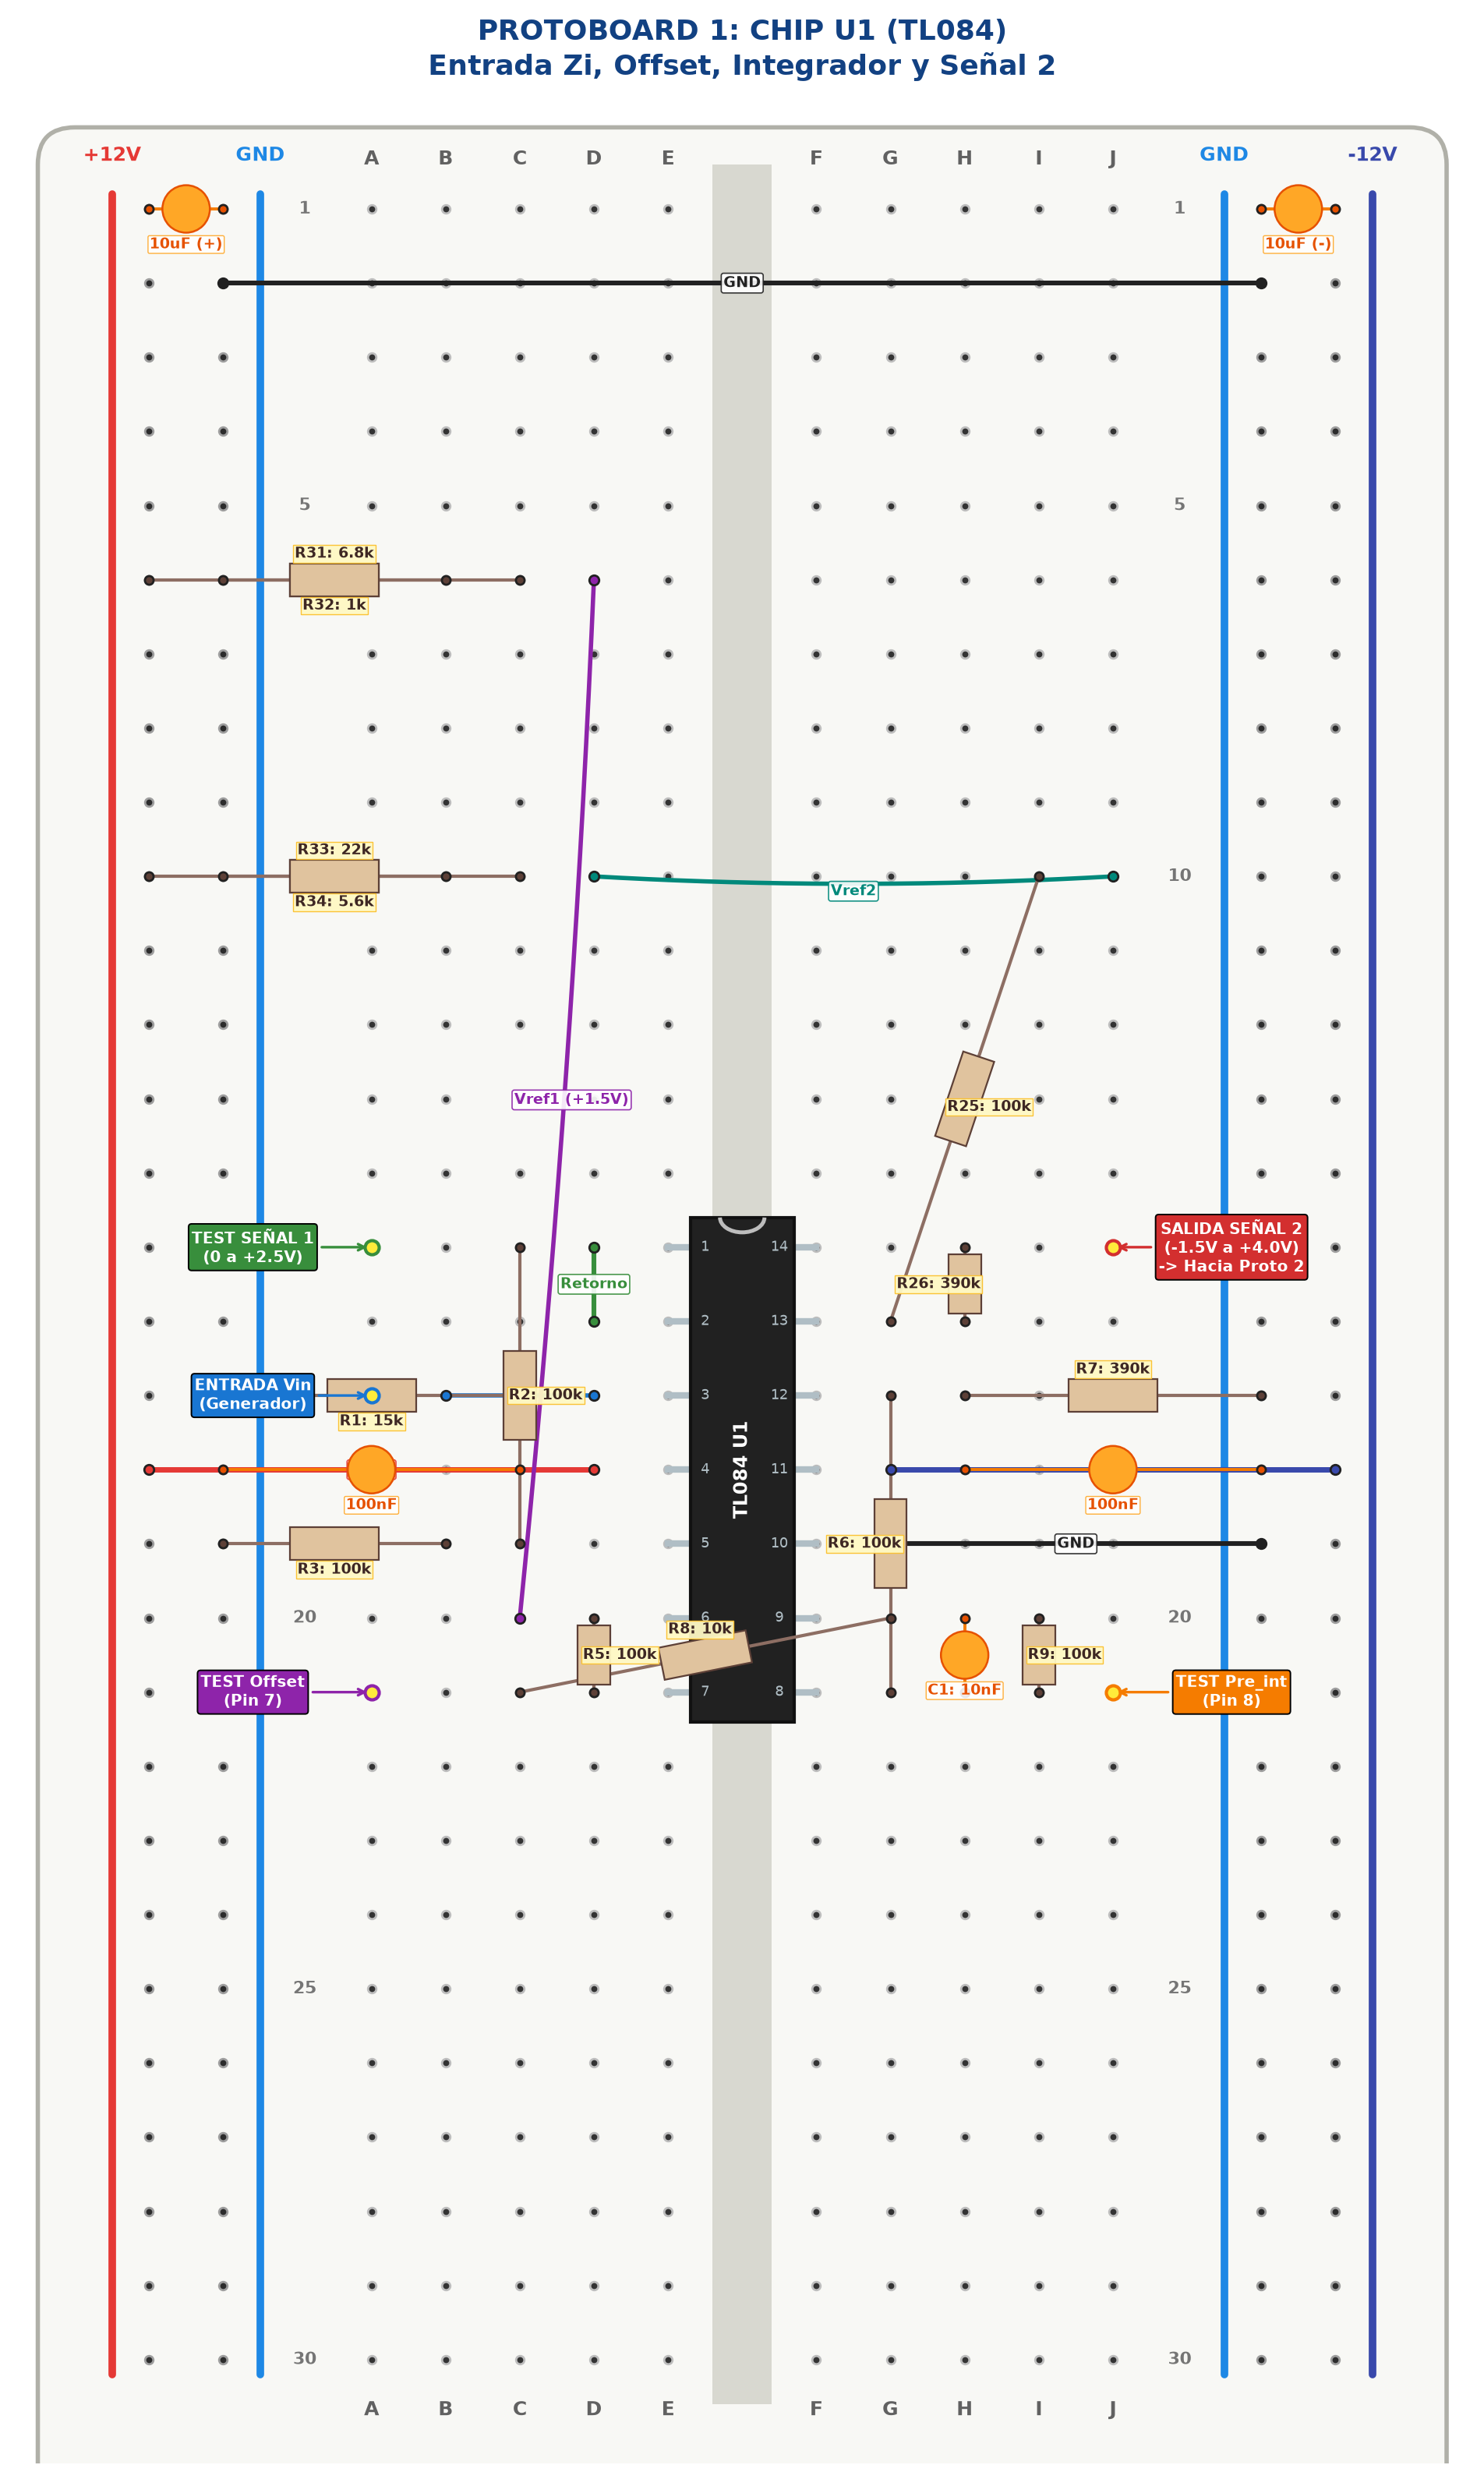
\includegraphics[height=15.8cm]{simulacion/proto_chip1.png}\\[4pt]
\captionof{figure}{Diagrama gráfico de conexionado literal en Protoboard 1 ($U_1$).}
\label{fig:proto_u1_diag}
\end{center}

\newpage

% ==================== PÁGINA 4: PROTOBOARD 1 (TABLA COORDENADAS) ====================
\subsection{Tabla de Coordenadas Físicas de Protoboard 1 (Chip \texorpdfstring{$U_1$}{U1})}

\begin{center}
\small
\renewcommand{\arraystretch}{1.08}
\begin{tabularx}{\textwidth}{l c c X}
\toprule
\textbf{Elemento} & \textbf{Desde (Orificio)} & \textbf{Hasta (Orificio)} & \textbf{Función / Detalle en el Circuito} \\
\midrule
\rowcolor{softgray} \textbf{CI $U_1$ (TL084)} & \texttt{E15} a \texttt{E21} (Pines 1--7) & \texttt{F21} a \texttt{F15} (Pines 8--14) & Cuádruple JFET DIP-14 sobre canal central (muesca arriba) \\
Jumper $+12\text{V}$ & Riel $+12\text{V}$ (izq, fila 18) & \texttt{D18} (Pin 4) & Alimentación positiva de $U_1$ \\
\rowcolor{softgray} Cap. Desacoplo & \texttt{C18} (Pin 4) & Riel GND (izq, fila 18) & Cerámico $\SI{100}{\nano\farad}$ (104) pegado a Pin 4 \\
Jumper $-12\text{V}$ & Riel $-12\text{V}$ (der, fila 18) & \texttt{G18} (Pin 11) & Alimentación negativa de $U_1$ \\
\rowcolor{softgray} Cap. Desacoplo & \texttt{H18} (Pin 11) & Riel GND (der, fila 18) & Cerámico $\SI{100}{\nano\farad}$ (104) pegado a Pin 11 \\
Puente de Masa & Riel GND izq. (fila 2) & Riel GND der. (fila 2) & Jumper negro grueso de equipotencialidad \\
Cap. Bulk $+12\text{V}$ & Riel $+12\text{V}$ (fila 1) & Riel GND izq. (fila 1) & Electrolítico $\SI{10}{\micro\farad} / \SI{25}{\volt}$ (positivo a $+12\text{V}$) \\
\rowcolor{softgray} Cap. Bulk $-12\text{V}$ & Riel GND der. (fila 1) & Riel $-12\text{V}$ (fila 1) & Electrolítico $\SI{10}{\micro\farad} / \SI{25}{\volt}$ (positivo a GND, negativo a $-12\text{V}$) \\
\midrule
\textbf{Generador $V_{in}$} & Conector externo (BNC) & \texttt{A17} & Señal cuadrada $4300\text{ Hz}$ ($0\text{ V}$ a $+2.5\text{ V}$) \\
\rowcolor{softgray} Jumper $V_{in}$ & \texttt{B17} & \texttt{D17} (Pin 3) & Conexión directa a entrada no inversora $U_{1A}$ \\
Resistencia $R_1$ & \texttt{C17} (Pin 3) & Riel GND izq. (fila 17) & $\SI{15}{\kilo\ohm}$ (Fija la impedancia de entrada $Z_i = \SI{15}{\kilo\ohm}$) \\
\rowcolor{softgray} Jumper Retorno & \texttt{D15} (Pin 1) & \texttt{D16} (Pin 2) & Retorno unitario seguidor (salida Pin 1 a inversora Pin 2) \\
\textbf{TEST SEÑAL 1} & \texttt{A15} & Punta de Osciloscopio & \textbf{Punto de Test S1}: Cuadrada $0\text{ V}$ a $+2.5\text{ V}$ simétrica \\
\midrule
Resistencia $R_2$ & \texttt{C15} (Pin 1) & \texttt{C19} (Pin 5) & $\SI{100}{\kilo\ohm}$ (Lleva Señal 1 a la entrada no inversora de $U_{1B}$) \\
\rowcolor{softgray} Resistencia $R_3$ & \texttt{B19} (Pin 5) & Riel GND izq. (fila 19) & $\SI{100}{\kilo\ohm}$ (Referencia a masa del sumador de offset) \\
Resistencia $R_{31}$ & Riel $+12\text{V}$ (fila 6) & \texttt{C6} & $\SI{6.8}{\kilo\ohm}$ (Divisor superior de referencia $V_{ref1}$) \\
\rowcolor{softgray} Resistencia $R_{32}$ & \texttt{B6} & Riel GND izq. (fila 6) & $\SI{1}{\kilo\ohm}$ (Divisor inferior de $V_{ref1} \implies +1.54\text{ V}$ en fila 6) \\
Jumper $V_{ref1}$ & \texttt{D6} & \texttt{C20} (Pin 6) & Lleva $V_{ref1}$ a la entrada inversora de $U_{1B}$ mediante $R_4$ \\
\rowcolor{softgray} Resistencia $R_5$ & \texttt{D20} (Pin 6) & \texttt{D21} (Pin 7) & $\SI{100}{\kilo\ohm}$ (Resistencia de realimentación del sumador $U_{1B}$) \\
\textbf{TEST Offset} & \texttt{A21} & Punta de Osciloscopio & Cuadrada con nivel medio desplazado hacia continua negativa \\
\midrule
Jumper Pin 10 & \texttt{G19} (Pin 10) & Riel GND der. (fila 19) & Entrada no inversora de $U_{1C}$ a masa ($0\text{ V}$) \\
\rowcolor{softgray} Resistencia $R_8$ & \texttt{C21} (Pin 7) & \texttt{G20} (Pin 9) & $\SI{10}{\kilo\ohm}$ (Resistencia de entrada del integrador Miller) \\
Capacitor $C_1$ & \texttt{H20} (Pin 9) & \texttt{H21} (Pin 8) & $\SI{10}{\nano\farad}$ poliéster/cerámico (Capacitor de integración Miller) \\
\rowcolor{softgray} Resistencia $R_9$ & \texttt{I20} (Pin 9) & \texttt{I21} (Pin 8) & $\SI{100}{\kilo\ohm}$ (Resistencia de amortiguación en paralelo con $C_1$) \\
\textbf{TEST Pre\_int} & \texttt{J21} & Punta de Osciloscopio & Triangular montada sobre nivel de continua positivo \\
\midrule
Resistencia $R_6$ & \texttt{G21} (Pin 8) & \texttt{G17} (Pin 12) & $\SI{100}{\kilo\ohm}$ (Conecta salida de integrador a entrada no inv. $U_{1D}$) \\
\rowcolor{softgray} Resistencia $R_7$ & \texttt{H17} (Pin 12) & Riel GND der. (fila 17) & $\SI{390}{\kilo\ohm}$ (Atenuador / divisor no inversor del centrador) \\
Resistencia $R_{33}$ & Riel $+12\text{V}$ (fila 10) & \texttt{C10} & $\SI{22}{\kilo\ohm}$ (o Preset $50\text{ k}\Omega$ W503 para calibración fina de continua) \\
\rowcolor{softgray} Resistencia $R_{34}$ & \texttt{B10} & Riel GND izq. (fila 10) & $\SI{5.6}{\kilo\ohm}$ (Divisor inferior de referencia $V_{ref2}$) \\
Jumper $V_{ref2}$ & \texttt{D10} & \texttt{J10} & Cable cruzado que lleva $V_{ref2}$ a la derecha de la placa \\
\rowcolor{softgray} Resistencia $R_{25}$ & \texttt{I10} & \texttt{G16} (Pin 13) & $\SI{100}{\kilo\ohm}$ (Entrada inversora del amplificador centrador $U_{1D}$) \\
Resistencia $R_{26}$ & \texttt{H16} (Pin 13) & \texttt{H15} (Pin 14) & $\SI{390}{\kilo\ohm}$ (Resistencia de realimentación del centrador $U_{1D}$) \\
\rowcolor{utnblue!15} \textbf{SALIDA SEÑAL 2} & \texttt{J15} (Pin 14) & \textbf{Cable a Protoboard 2} & \textbf{Punto de Test S2}: Triangular $\SI{-1.5}{\volt}$ a $\SI{+4.0}{\volt}$ ($V_{pp}=\SI{5.5}{\volt}$) \\
\bottomrule
\end{tabularx}\\[4pt]
\captionof{table}{Tabla de conexionado detallado de Protoboard 1 ($U_1$).}
\end{center}

\newpage

% ==================== PÁGINA 5: PROTOBOARD 2 (DIAGRAMA) ====================
\section{Protoboard 2: Esquema Gráfico Literal (Chip \texorpdfstring{$U_2$}{U2})}

\begin{center}
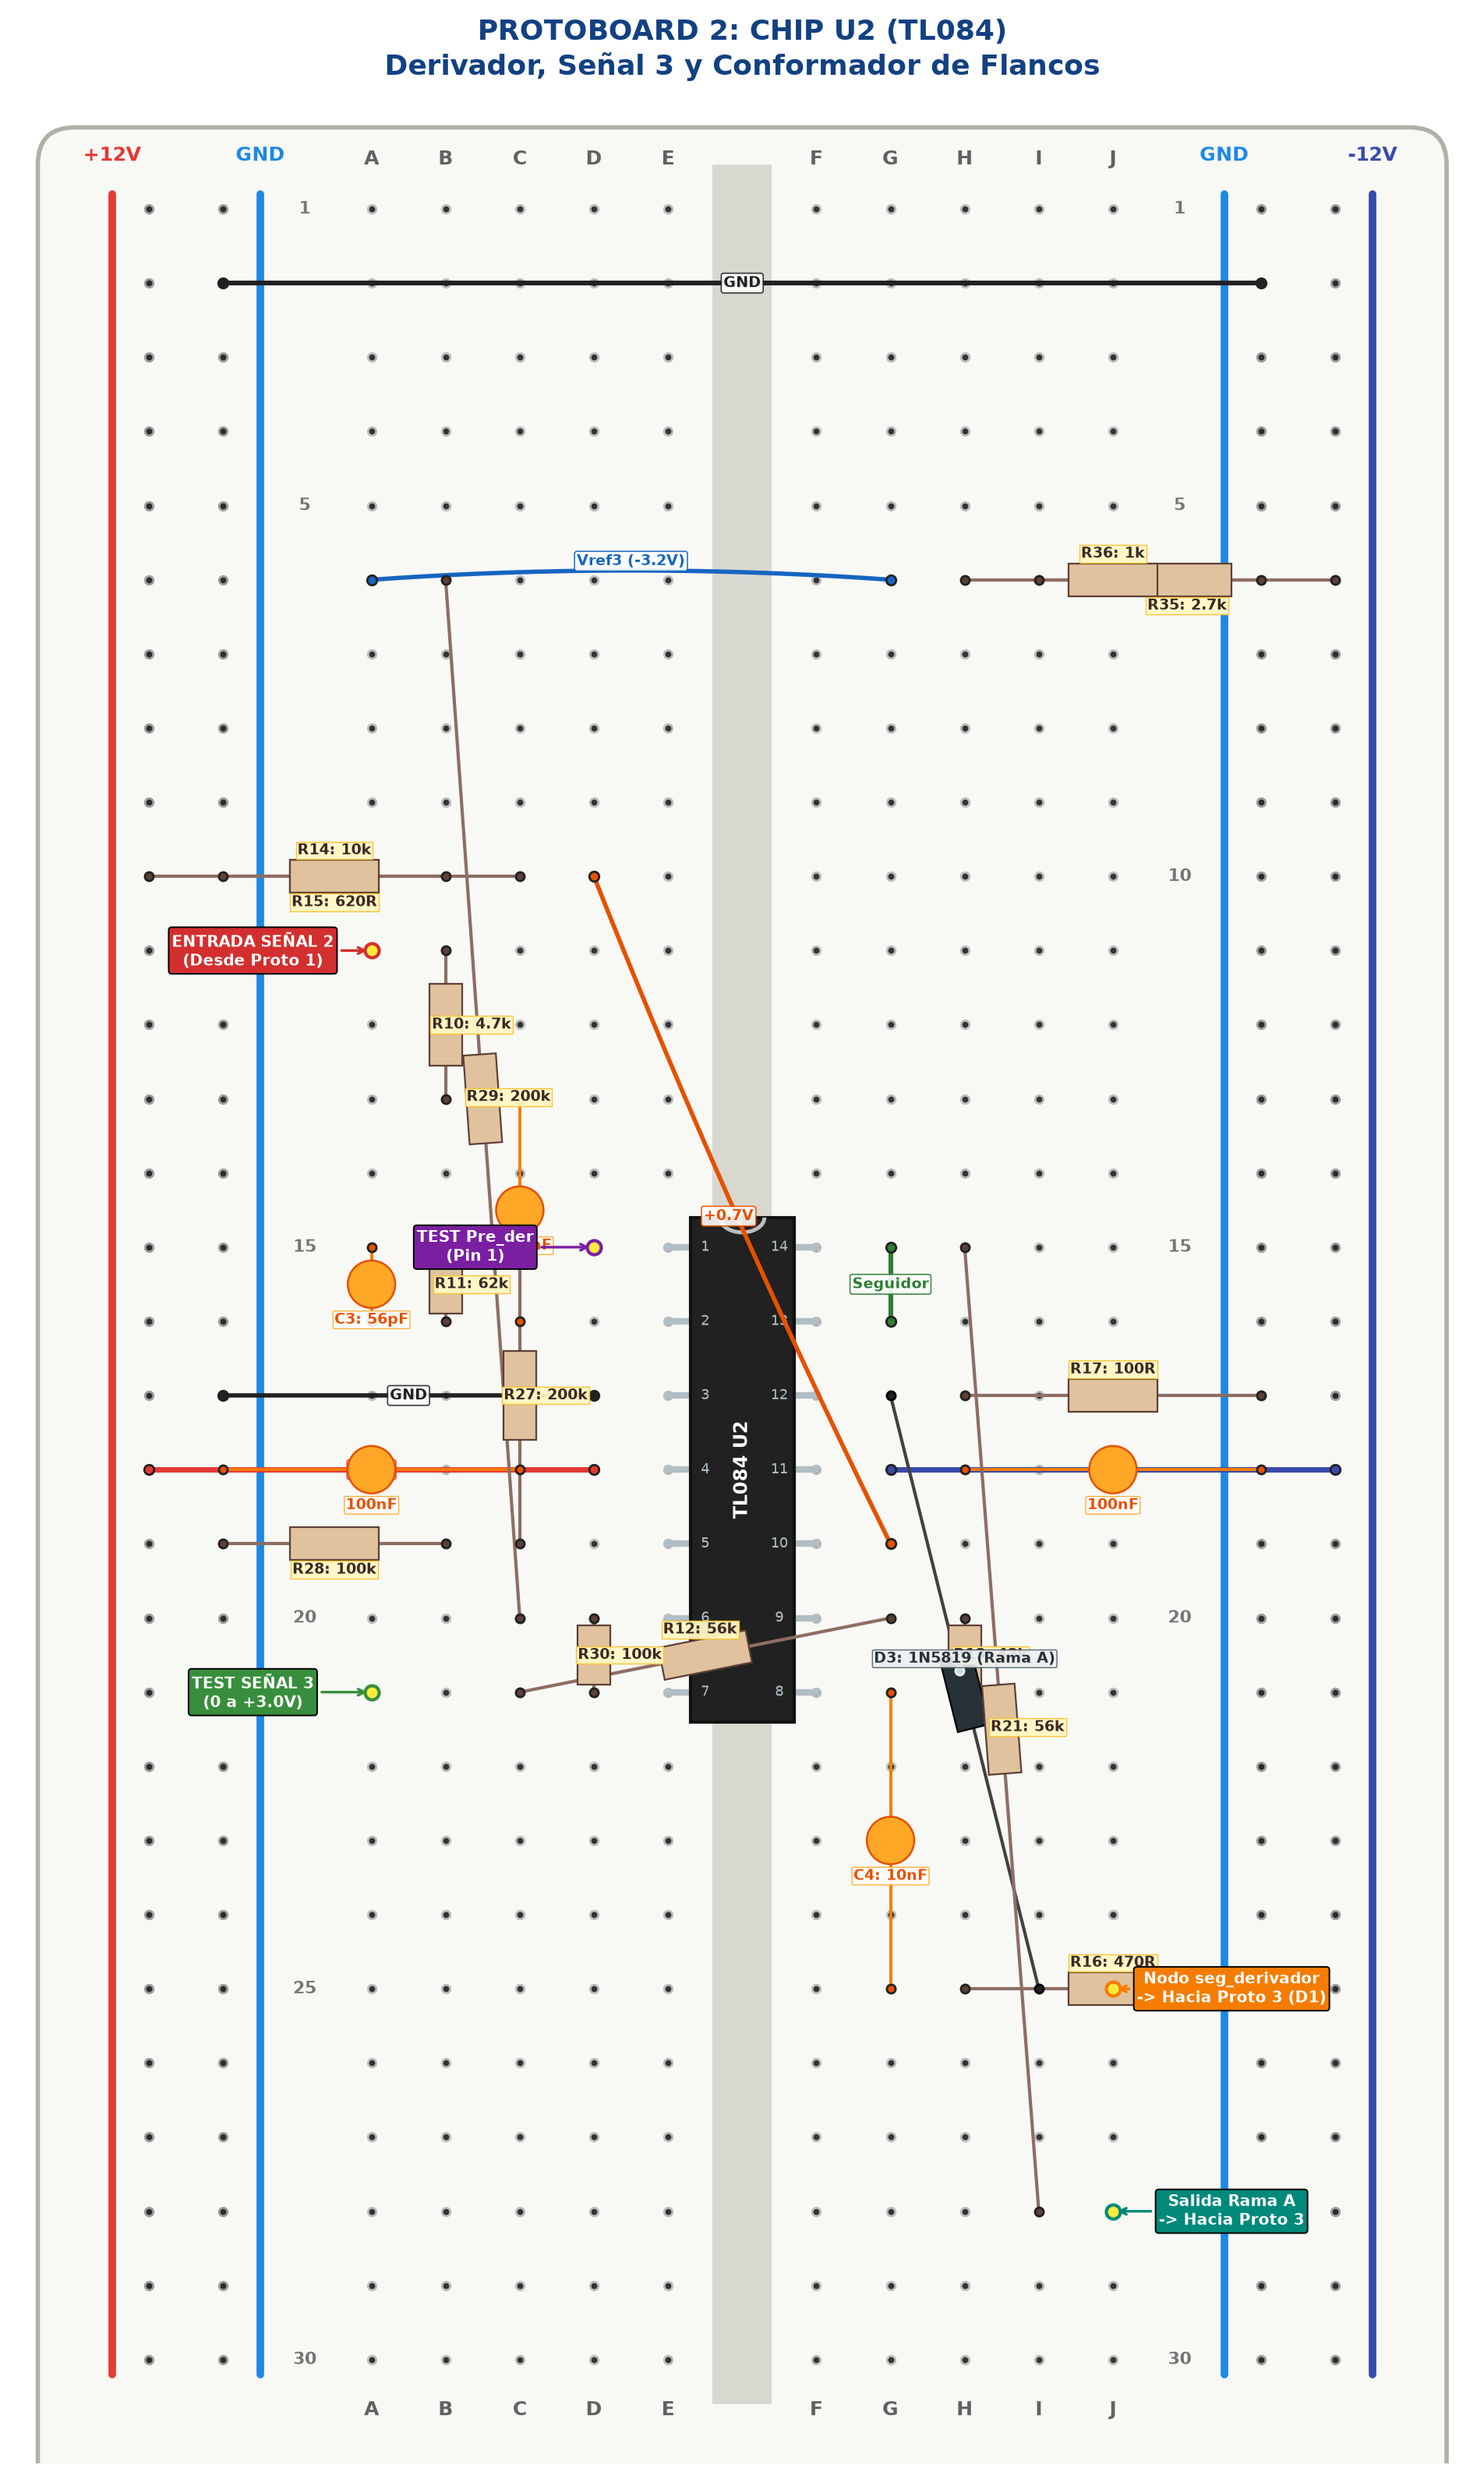
\includegraphics[height=15.8cm]{simulacion/proto_chip2.png}\\[4pt]
\captionof{figure}{Diagrama gráfico de conexionado literal en Protoboard 2 ($U_2$).}
\label{fig:proto_u2_diag}
\end{center}

\newpage

% ==================== PÁGINA 6: PROTOBOARD 2 (TABLA COORDENADAS) ====================
\subsection{Tabla de Coordenadas Físicas de Protoboard 2 (Chip \texorpdfstring{$U_2$}{U2})}

\begin{center}
\small
\renewcommand{\arraystretch}{1.08}
\begin{tabularx}{\textwidth}{l c c X}
\toprule
\textbf{Elemento} & \textbf{Desde (Orificio)} & \textbf{Hasta (Orificio)} & \textbf{Función / Detalle en el Circuito} \\
\midrule
\rowcolor{softgray} \textbf{CI $U_2$ (TL084)} & \texttt{E15} a \texttt{E21} (Pines 1--7) & \texttt{F21} a \texttt{F15} (Pines 8--14) & Cuádruple JFET DIP-14 sobre canal central (muesca arriba) \\
Jumper $+12\text{V}$ & Riel $+12\text{V}$ (izq, fila 18) & \texttt{D18} (Pin 4) & Alimentación positiva de $U_2$ \\
\rowcolor{softgray} Cap. Desacoplo & \texttt{C18} (Pin 4) & Riel GND (izq, fila 18) & Cerámico $\SI{100}{\nano\farad}$ (104) pegado a Pin 4 \\
Jumper $-12\text{V}$ & Riel $-12\text{V}$ (der, fila 18) & \texttt{G18} (Pin 11) & Alimentación negativa de $U_2$ \\
\rowcolor{softgray} Cap. Desacoplo & \texttt{H18} (Pin 11) & Riel GND (der, fila 18) & Cerámico $\SI{100}{\nano\farad}$ (104) pegado a Pin 11 \\
Puente de Masa & Riel GND izq. (fila 2) & Riel GND der. (fila 2) & Jumper negro grueso de equipotencialidad \\
\midrule
\textbf{Entrada Señal 2} & Desde Proto 1 (\texttt{J15}) & \texttt{A11} & Llega la onda triangular de $\SI{-1.5}{\volt}$ a $\SI{+4.0}{\volt}$ \\
\rowcolor{softgray} Resistencia $R_{10}$ & \texttt{B11} & \texttt{B13} & $\SI{4.7}{\kilo\ohm}$ (Resistencia serie de limitación para el derivador) \\
Capacitor $C_2$ & \texttt{C13} & \texttt{C16} (Pin 2) & $\SI{1}{\nano\farad}$ cerámico/poliéster (Capacitor serie derivador Miller) \\
\rowcolor{softgray} Jumper Pin 3 & \texttt{D17} (Pin 3) & Riel GND izq. (fila 17) & Entrada no inversora de $U_{2A}$ a masa ($0\text{ V}$) \\
Resistencia $R_{11}$ & \texttt{B15} (Pin 1) & \texttt{B16} (Pin 2) & $\SI{62}{\kilo\ohm}$ (Resistencia de realimentación del derivador Miller) \\
\rowcolor{softgray} Capacitor $C_3$ & \texttt{A15} (Pin 1) & \texttt{A16} (Pin 2) & $\SI{56}{\pico\farad}$ cerámico (Compensación de estabilidad contra sobrepicos) \\
\textbf{TEST Pre\_der} & \texttt{D15} & Punta de Osciloscopio & Cuadrada simétrica $\pm 3\text{ V}$ libre de oscilaciones \\
\midrule
Resistencia $R_{27}$ & \texttt{C15} (Pin 1) & \texttt{C19} (Pin 5) & $\SI{200}{\kilo\ohm}$ (Conecta salida de derivador a entrada no inv. $U_{2B}$) \\
\rowcolor{softgray} Resistencia $R_{28}$ & \texttt{B19} (Pin 5) & Riel GND izq. (fila 19) & $\SI{100}{\kilo\ohm}$ (Referencia a masa del conformador de Señal 3) \\
Resistencia $R_{35}$ & Riel $-12\text{V}$ (der, fila 6) & \texttt{I6} & $\SI{2.7}{\kilo\ohm}$ (Divisor superior de referencia negativa $V_{ref3}$) \\
\rowcolor{softgray} Resistencia $R_{36}$ & \texttt{H6} & Riel GND der. (fila 6) & $\SI{1}{\kilo\ohm}$ (Divisor inferior de $V_{ref3} \implies -3.24\text{ V}$ en fila 6) \\
Jumper $V_{ref3}$ & \texttt{G6} & \texttt{A6} & Lleva $V_{ref3}$ desde el lado derecho hacia la columna izquierda \\
\rowcolor{softgray} Resistencia $R_{29}$ & \texttt{B6} & \texttt{C20} (Pin 6) & $\SI{200}{\kilo\ohm}$ (Entrada inversora del conformador $U_{2B}$) \\
Resistencia $R_{30}$ & \texttt{D20} (Pin 6) & \texttt{D21} (Pin 7) & $\SI{100}{\kilo\ohm}$ (Realimentación conformador de nivel de continua) \\
\rowcolor{utnblue!15} \textbf{SALIDA SEÑAL 3} & \texttt{A21} (Pin 7) & \textbf{Punto de Test S3} & \textbf{Señal 3}: Cuadrada unipolar de $\SI{0.0}{\volt}$ a $\SI{+3.0}{\volt}$ ($V_{pp}=\SI{3.0}{\volt}$) \\
\midrule
Resistencia $R_{14}$ & Riel $+12\text{V}$ (fila 10) & \texttt{C10} & $\SI{10}{\kilo\ohm}$ (Divisor superior de umbral $+0.7\text{ V}$) \\
\rowcolor{softgray} Resistencia $R_{15}$ & \texttt{B10} & Riel GND izq. (fila 10) & $\SI{620}{\ohm}$ (Divisor inferior de umbral $+0.7\text{ V}$) \\
Jumper Umbral & \texttt{D10} & \texttt{G19} (Pin 10) & Conecta el umbral de $+0.7\text{ V}$ a la entrada no inv. de $U_{2C}$ \\
\rowcolor{softgray} Resistencia $R_{12}$ & \texttt{C21} (Pin 7) & \texttt{G20} (Pin 9) & $\SI{56}{\kilo\ohm}$ (Entrada inversora del inversor conformador $U_{2C}$) \\
Resistencia $R_{13}$ & \texttt{H20} (Pin 9) & \texttt{H21} (Pin 8) & $\SI{43}{\kilo\ohm}$ (Realimentación del inversor $U_{2C}$) \\
\midrule
Capacitor $C_4$ & \texttt{G21} (Pin 8) & \texttt{G25} & $\SI{10}{\nano\farad}$ (Derivador pasivo generador de picos bipolares) \\
\rowcolor{softgray} Resistencia $R_{16}$ & \texttt{H25} & Riel GND der. (fila 25) & $\SI{470}{\ohm}$ (Resistencia de carga del derivador pasivo) \\
\textbf{seg\_derivador} & \texttt{J25} & \textbf{Cable a Protoboard 3} & \textbf{Cable de picos}: Lleva los pulsos bipolares hacia el diodo $D_1$ \\
\rowcolor{softgray} Diodo $D_3$ & \texttt{I25} (Ánodo) & \texttt{G17} (Cátodo/Franja) & Schottky 1N5819 (Rectificador de picos positivos --- Rama A) \\
Resistencia $R_{17}$ & \texttt{H17} (Pin 12) & Riel GND der. (fila 17) & $\SI{100}{\ohm}$ (Carga de cátodo de $D_3$ hacia masa) \\
\rowcolor{softgray} Jumper Seguidor & \texttt{G16} (Pin 13) & \texttt{G15} (Pin 14) & Buffer unitario de precisión $U_{2D}$ (Pin 13 a Pin 14) \\
Resistencia $R_{21}$ & \texttt{H15} (Pin 14) & \texttt{I28} & $\SI{56}{\kilo\ohm}$ (Resistencia de salida del sumador Rama A) \\
\rowcolor{utnblue!15} \textbf{Salida Rama A} & \texttt{J28} & \textbf{Cable a Protoboard 3} & \textbf{Cable al Pin 5 de $U_3$}: Señal rectificada de la Rama A \\
\bottomrule
\end{tabularx}\\[4pt]
\captionof{table}{Tabla de conexionado detallado de Protoboard 2 ($U_2$).}
\end{center}

\newpage

% ==================== PÁGINA 7: PROTOBOARD 3 (DIAGRAMA) ====================
\section{Protoboard 3: Esquema Gráfico Literal (Chip \texorpdfstring{$U_3$}{U3})}

\begin{center}
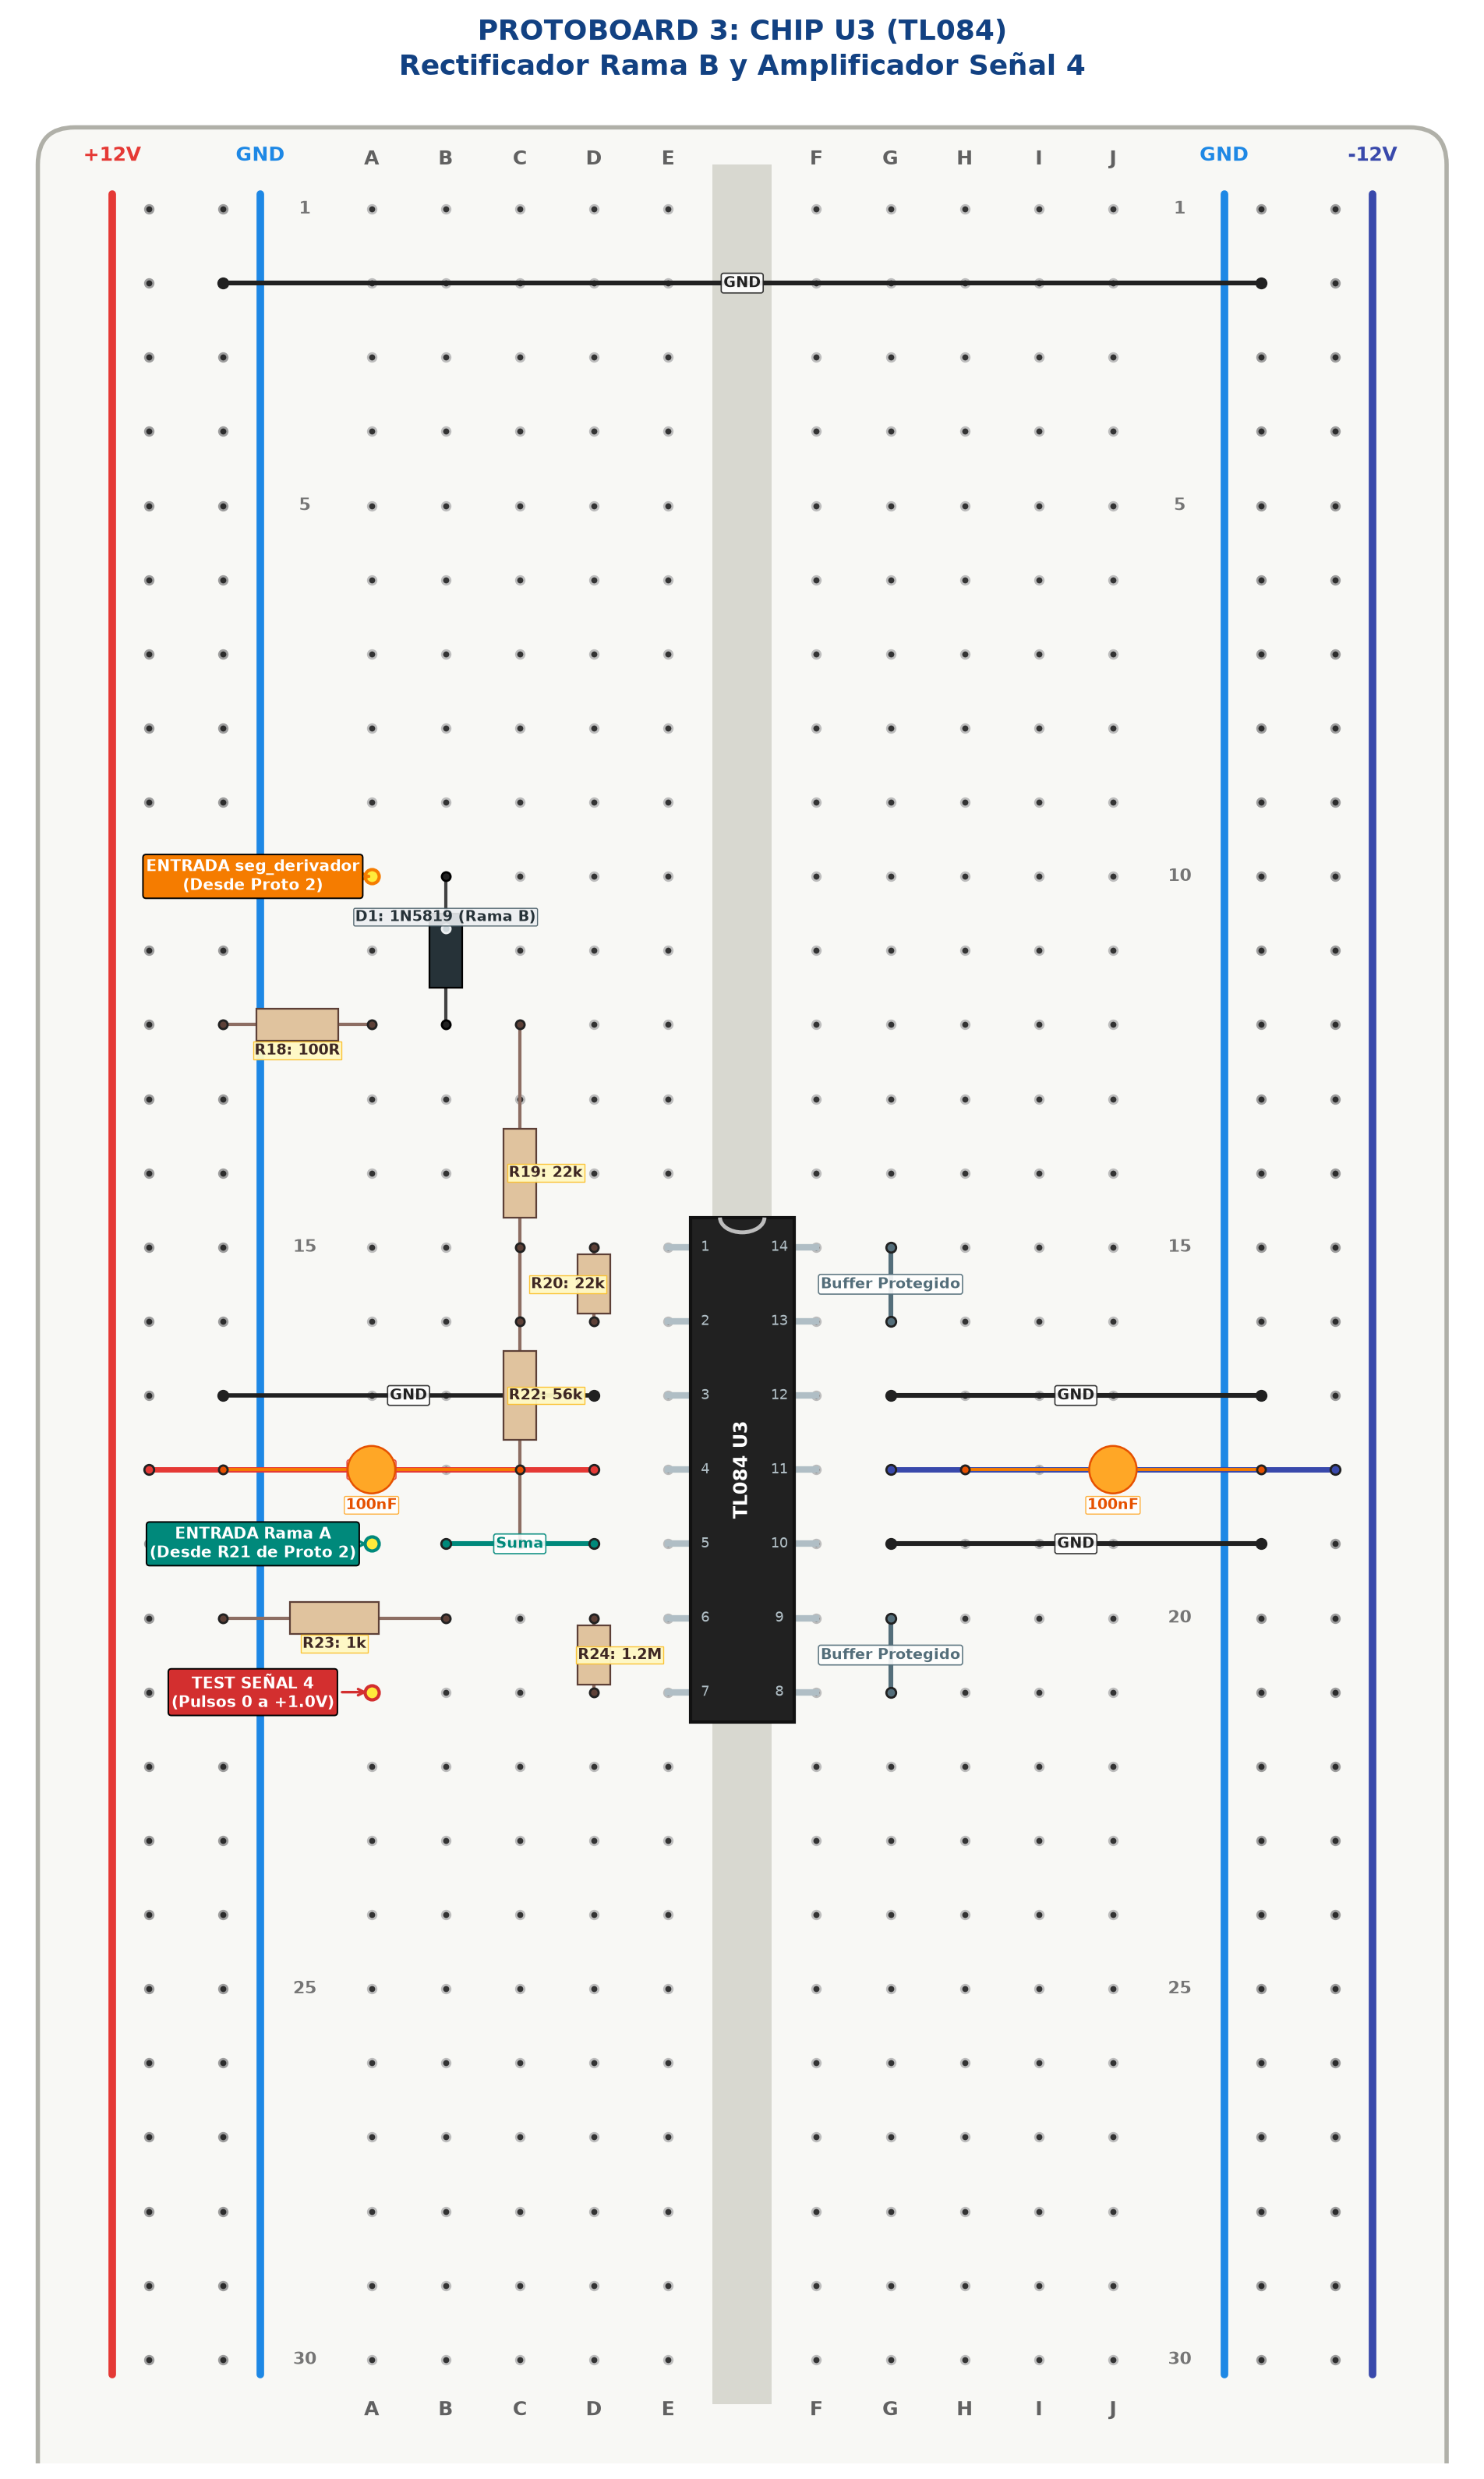
\includegraphics[height=15.8cm]{simulacion/proto_chip3.png}\\[4pt]
\captionof{figure}{Diagrama gráfico de conexionado literal en Protoboard 3 ($U_3$).}
\label{fig:proto_u3_diag}
\end{center}

\newpage

% ==================== PÁGINA 8: PROTOBOARD 3 (TABLA COORDENADAS) ====================
\subsection{Tabla de Coordenadas Físicas de Protoboard 3 (Chip \texorpdfstring{$U_3$}{U3})}

\begin{center}
\small
\renewcommand{\arraystretch}{1.08}
\begin{tabularx}{\textwidth}{l c c X}
\toprule
\textbf{Elemento} & \textbf{Desde (Orificio)} & \textbf{Hasta (Orificio)} & \textbf{Función / Detalle en el Circuito} \\
\midrule
\rowcolor{softgray} \textbf{CI $U_3$ (TL084)} & \texttt{E15} a \texttt{E21} (Pines 1--7) & \texttt{F21} a \texttt{F15} (Pines 8--14) & Cuádruple JFET DIP-14 sobre canal central (muesca arriba) \\
Jumper $+12\text{V}$ & Riel $+12\text{V}$ (izq, fila 18) & \texttt{D18} (Pin 4) & Alimentación positiva de $U_3$ \\
\rowcolor{softgray} Cap. Desacoplo & \texttt{C18} (Pin 4) & Riel GND (izq, fila 18) & Cerámico $\SI{100}{\nano\farad}$ (104) pegado a Pin 4 \\
Jumper $-12\text{V}$ & Riel $-12\text{V}$ (der, fila 18) & \texttt{G18} (Pin 11) & Alimentación negativa de $U_3$ \\
\rowcolor{softgray} Cap. Desacoplo & \texttt{H18} (Pin 11) & Riel GND (der, fila 18) & Cerámico $\SI{100}{\nano\farad}$ (104) pegado a Pin 11 \\
Puente de Masa & Riel GND izq. (fila 2) & Riel GND der. (fila 2) & Jumper negro grueso de equipotencialidad \\
\midrule
\textbf{Entrada seg\_derivador} & Desde Proto 2 (\texttt{J25}) & \texttt{A10} & Llegan los picos bipolares de derivación \\
\rowcolor{softgray} Diodo $D_1$ & \texttt{B10} (Cátodo/Franja) & \texttt{B12} (Ánodo) & Schottky 1N5819 (Conduce en picos negativos --- Rama B) \\
Resistencia $R_{18}$ & \texttt{A12} & Riel GND izq. (fila 12) & $\SI{100}{\ohm}$ (Resistencia de polarización de ánodo a masa) \\
\rowcolor{softgray} Resistencia $R_{19}$ & \texttt{C12} & \texttt{C16} (Pin 2) & $\SI{22}{\kilo\ohm}$ (Entrada inversora del rectificador inversor $U_{3A}$) \\
Jumper Pin 3 & \texttt{D17} (Pin 3) & Riel GND izq. (fila 17) & Entrada no inversora de $U_{3A}$ a masa ($0\text{ V}$) \\
\rowcolor{softgray} Resistencia $R_{20}$ & \texttt{D16} (Pin 2) & \texttt{D15} (Pin 1) & $\SI{22}{\kilo\ohm}$ (Realimentación unitaria inversora de $U_{3A}$) \\
Resistencia $R_{22}$ & \texttt{C15} (Pin 1) & \texttt{C19} (Pin 5) & $\SI{56}{\kilo\ohm}$ (Salida Rama B hacia el nodo común \texttt{rectificador}) \\
\midrule
\textbf{Entrada Rama A} & Desde Proto 2 (\texttt{J28}) & \texttt{A19} & Llega la señal rectificada proveniente de $R_{21}$ \\
\rowcolor{softgray} Jumper Suma & \texttt{B19} & \texttt{D19} (Pin 5) & Une la Rama A con la Rama B en la entrada no inv. $U_{3B}$ \\
Resistencia $R_{23}$ & \texttt{B20} (Pin 6) & Riel GND izq. (fila 20) & $\SI{1}{\kilo\ohm}$ (Resistencia de ganancia a masa del amplificador de salida) \\
\rowcolor{softgray} Resistencia $R_{24}$ & \texttt{D20} (Pin 6) & \texttt{D21} (Pin 7) & $\SI{1.2}{\mega\ohm}$ (Resistencia de realimentación del amplificador $U_{3B}$) \\
\rowcolor{darkred!15} \textbf{SALIDA SEÑAL 4} & \texttt{A21} (Pin 7) & \textbf{Punto de Test S4} & \textbf{Señal 4}: Tren de pulsos positivos de $\SI{0.0}{\volt}$ a $\SI{+1.0}{\volt}$ \\
\midrule
\multicolumn{4}{l}{\textbf{Terminación y Protección contra Oscilaciones de Operacionales Libres (Texas Instruments):}} \\
\rowcolor{softgray} Jumper Pin 10 a GND & \texttt{G19} (Pin 10) & Riel GND der. (fila 19) & Conecta entrada no inversora de $U_{3C}$ a masa ($0\text{ V}$) \\
Jumper Buffer $U_{3C}$ & \texttt{G21} (Pin 8) & \texttt{G20} (Pin 9) & Conecta salida a entrada inversora (Buffer unitario a $0\text{ V}$) \\
\rowcolor{softgray} Jumper Pin 12 a GND & \texttt{G17} (Pin 12) & Riel GND der. (fila 17) & Conecta entrada no inversora de $U_{3D}$ a masa ($0\text{ V}$) \\
Jumper Buffer $U_{3D}$ & \texttt{G15} (Pin 14) & \texttt{G16} (Pin 13) & Conecta salida a entrada inversora (Buffer unitario a $0\text{ V}$) \\
\bottomrule
\end{tabularx}\\[4pt]
\captionof{table}{Tabla de conexionado detallado de Protoboard 3 ($U_3$).}
\end{center}

\newpage

% ==================== PÁGINA 9: FORMAS DE ONDA Y PUNTOS DE TEST ====================
\section{Formas de Onda Esperadas y Puntos de Prueba (Osciloscopio)}

\begin{figure}[H]
\centering
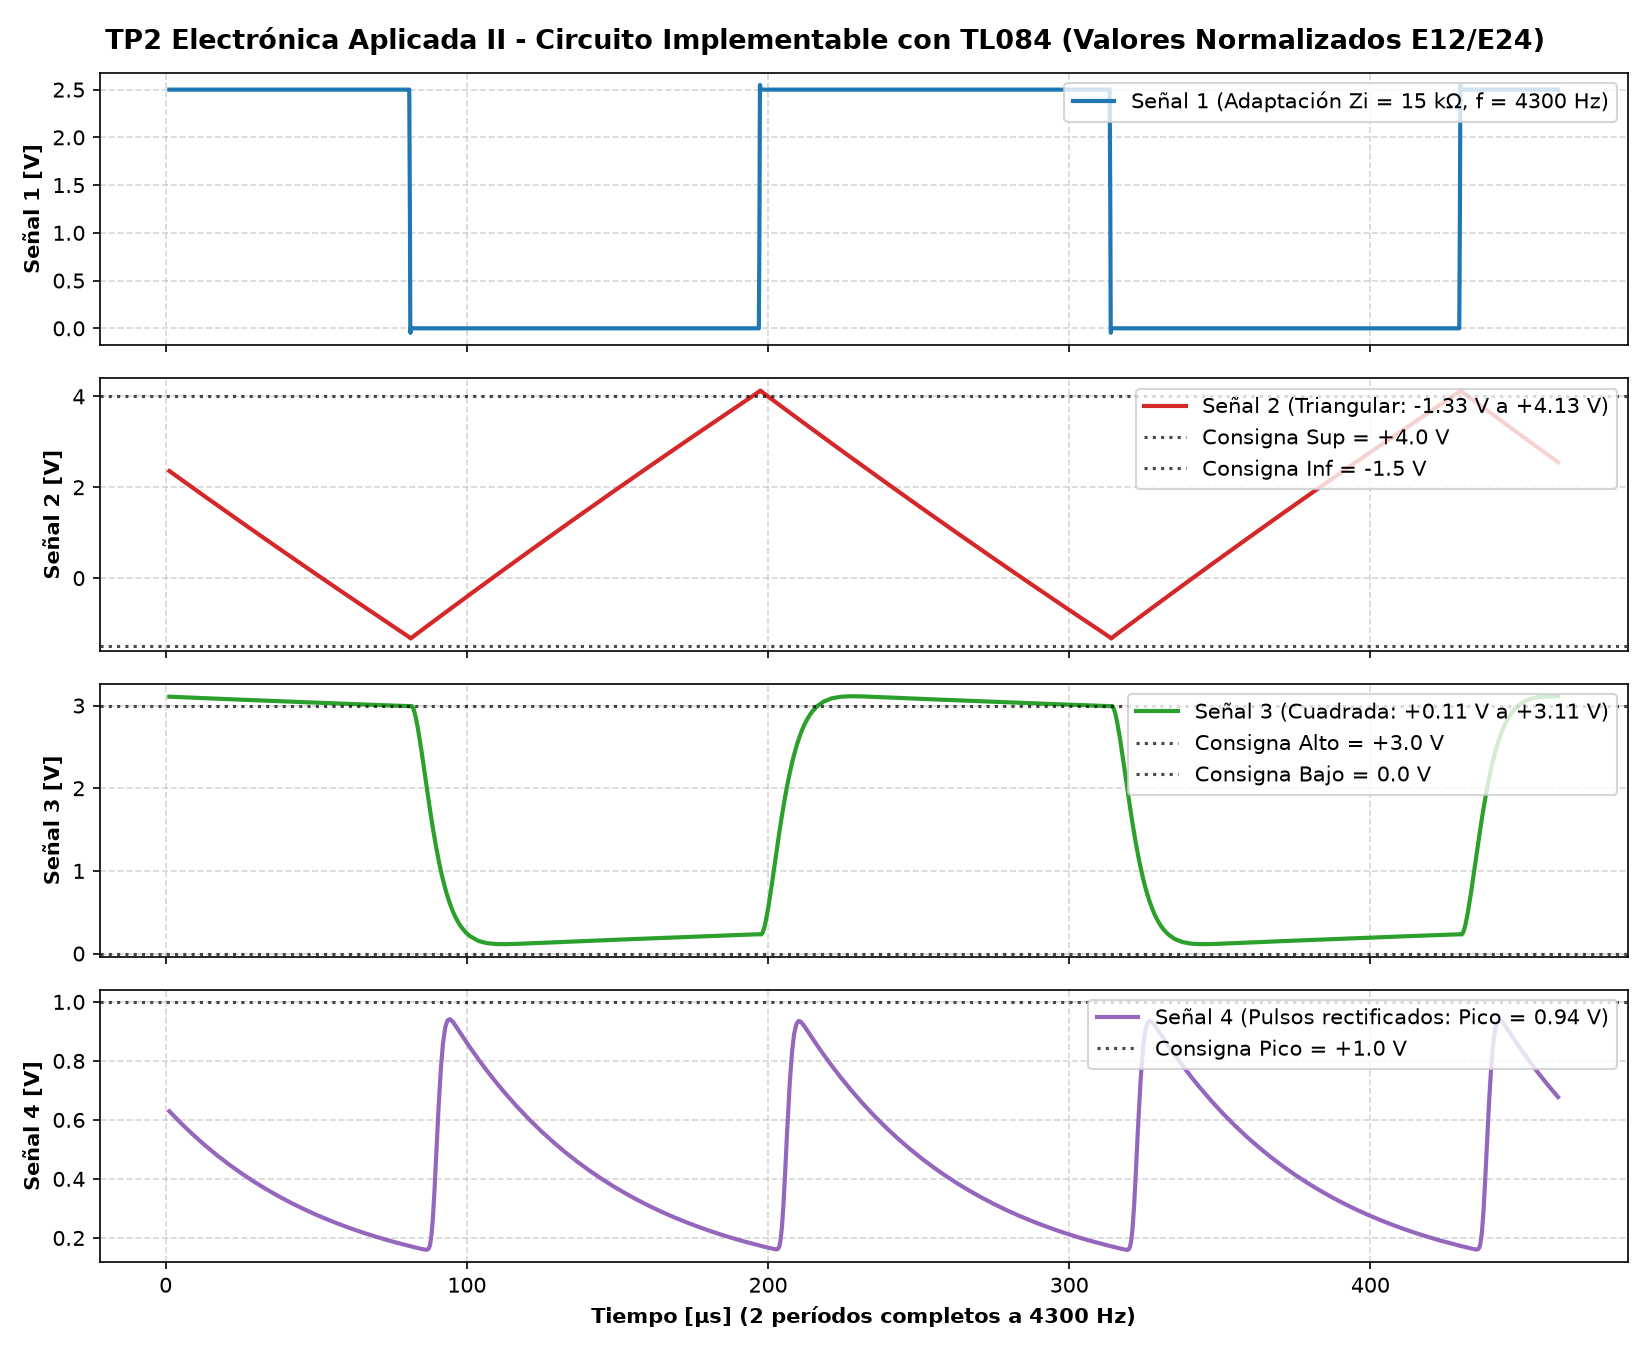
\includegraphics[width=0.96\textwidth]{simulacion/senales_TL084.png}
\caption{Verificación transitoria completa con el macromodelo del TL084 y componentes normalizados.}
\label{fig:curvas_tl084}
\end{figure}

\begin{table}[H]
\centering
\small
\renewcommand{\arraystretch}{1.25}
\begin{tabularx}{\textwidth}{l l c c c X}
\toprule
\textbf{Señal / Punto de Test} & \textbf{Ubicación Física} & \textbf{$V_{min}$} & \textbf{$V_{max}$} & \textbf{$V_{pp}$} & \textbf{Forma de Onda Esperada} \\
\midrule
\rowcolor{softgray} \textbf{Señal 1 (Adaptacion\_Zi)} & Pin 1 ($U_1$) / \texttt{A15} & $\SI{0.0}{\volt}$ & $\SI{+2.5}{\volt}$ & $\SI{2.5}{\volt}$ & Cuadrada simétrica $\SI{4300}{\hertz}$ ($Z_{in} = \SI{15}{\kilo\ohm}$). \\
\textbf{Nodo Offset} & Pin 7 ($U_1$) / \texttt{A21} & $\SI{-1.5}{\volt}$ & $\SI{+1.0}{\volt}$ & $\SI{2.5}{\volt}$ & Cuadrada con nivel medio $\approx \SI{-0.25}{\volt}$. \\
\rowcolor{softgray} \textbf{Nodo Pre\_int} & Pin 8 ($U_1$) / \texttt{J21} & $\SI{+2.1}{\volt}$ & $\SI{+3.5}{\volt}$ & $\SI{1.45}{\volt}$ & Triangular montada sobre continua. \\
\textbf{Señal 2 (Triangular)} & Pin 14 ($U_1$) / \texttt{J15} & $\SI{-1.3}{\volt} \approx \SI{-1.5}{\volt}$ & $\SI{+4.1}{\volt} \approx \SI{+4.0}{\volt}$ & $\SI{5.5}{\volt}$ & Triangular centrada según consigna del TP. \\
\rowcolor{softgray} \textbf{Nodo Pre\_der} & Pin 1 ($U_2$) / \texttt{D15} & $\SI{-3.0}{\volt}$ & $\SI{+3.0}{\volt}$ & $\SI{6.0}{\volt}$ & Cuadrada simétrica libre de sobrepicos. \\
\textbf{Señal 3 (Cuadrada)} & Pin 7 ($U_2$) / \texttt{A21} & $\SI{0.1}{\volt} \approx \SI{0.0}{\volt}$ & $\SI{+3.1}{\volt} \approx \SI{+3.0}{\volt}$ & $\SI{3.0}{\volt}$ & Cuadrada unipolar $\SI{0}{\volt}$ a $\SI{+3}{\volt}$. \\
\rowcolor{softgray} \textbf{Nodo seg\_derivador} & Fila 25 / \texttt{J25} & $\SI{-0.65}{\volt}$ & $\SI{+0.65}{\volt}$ & $\SI{1.3}{\volt}$ & Picos bipolares en cada flanco. \\
\textbf{Señal 4 (Pulsos rectificados)} & Pin 7 ($U_3$) / \texttt{A21} & $\SI{0.15}{\volt} \approx \SI{0.0}{\volt}$ & $\SI{+0.95}{\volt} \approx \SI{+1.0}{\volt}$ & $\SI{0.8}{\volt}$ & Picos exponenciales unipolares positivos. \\
\bottomrule
\end{tabularx}
\caption{Valores y puntos de prueba de verificación rápida en laboratorio.}
\end{table}

\newpage

% ==================== PÁGINA 10: LISTA DE MATERIALES (BOM) ====================
\section{Lista Consolidada de Materiales (BOM de Compras / Pañol)}

Todas las resistencias son de \textbf{$1/4\text{ W}$ ($0.25\text{ W}$)} al $\pm 1\%$ o $\pm 5\%$:

\begin{table}[H]
\centering
\small
\renewcommand{\arraystretch}{1.2}
\begin{tabularx}{\textwidth}{l c l X}
\toprule
\textbf{Componente} & \textbf{Cant.} & \textbf{Valor / Código} & \textbf{Designación en el Circuito} \\
\midrule
\rowcolor{softgray} \textbf{Circuitos Integrados} & 3 & \textbf{TL084CN (DIP-14)} & $U_1$, $U_2$, $U_3$ (Operacionales cuádruples JFET) \\
\textbf{Diodos Rápidos} & 2 & \textbf{1N5819 o BAT48} & $D_1, D_3$ (Diodos Schottky para el rectificador) \\
\rowcolor{softgray} \textbf{Preset Multivueltas} & 1 & \textbf{$50\text{ k}\Omega$ (W503)} & Ajuste fino de continua Señal 2 (en divisor $V_{ref2}$) \\
\midrule
\multirow{10}{*}{\textbf{Resistencias ($1/4\text{ W}$)}} 
& 2 & $\SI{100}{\ohm}$ & $R_{17}, R_{18}$ \\
& 1 & $\SI{470}{\ohm}$ & $R_{16}$ \\
& 1 & $\SI{620}{\ohm}$ (E24) & $R_{15}$ \\
& 3 & $\SI{1}{\kilo\ohm}$ & $R_{23}, R_{32}, R_{36}$ \\
& 1 & $\SI{2.7}{\kilo\ohm}$ (E24) & $R_{35}$ \\
& 1 & $\SI{4.7}{\kilo\ohm}$ & $R_{10}$ \\
& 1 & $\SI{5.6}{\kilo\ohm}$ & $R_{34}$ \\
& 1 & $\SI{6.8}{\kilo\ohm}$ & $R_{31}$ \\
& 2 & $\SI{10}{\kilo\ohm}$ & $R_8, R_{14}$ \\
& 1 & $\SI{15}{\kilo\ohm}$ & $R_1$ (Impedancia de entrada $Z_i$) \\
& 2 & $\SI{22}{\kilo\ohm}$ & $R_{19}, R_{20}$ \\
& 1 & $\SI{22}{\kilo\ohm}$ o preset & $R_{33}$ (Calibración Señal 2) \\
& 1 & $\SI{43}{\kilo\ohm}$ (E24) & $R_{13}$ \\
& 3 & $\SI{56}{\kilo\ohm}$ & $R_{12}, R_{21}, R_{22}$ \\
& 1 & $\SI{62}{\kilo\ohm}$ (E24) & $R_{11}$ \\
& 11 & $\SI{100}{\kilo\ohm}$ & $R_2, R_3, R_4, R_5, R_6, R_9, R_{25}, R_{28}, R_{30}$ (+ 2 para series) \\
& 2 & $\SI{200}{\kilo\ohm}$ (E24) & $R_{27}, R_{29}$ (o dos de $100\text{ k}\Omega$ en serie) \\
& 2 & $\SI{390}{\kilo\ohm}$ & $R_7, R_{26}$ (o $360\text{ k}\Omega + 20\text{ k}\Omega$ en serie) \\
& 1 & $\SI{1.2}{\mega\ohm}$ & $R_{24}$ (o $1\text{ M}\Omega + 200\text{ k}\Omega$) \\
\midrule
\multirow{4}{*}{\textbf{Capacitores Señal}}
& 1 & $\SI{56}{\pico\farad}$ (Cerámico) & $C_3$ (Compensación de sobrepico en derivador) \\
& 1 & $\SI{1}{\nano\farad}$ (Cerámico / Poliéster) & $C_2$ (Derivador de entrada) \\
& 2 & $\SI{10}{\nano\farad}$ (Poliéster / Cerámico) & $C_1$ (Integrador), $C_4$ (Diferenciador de pulsos) \\
\midrule
\multirow{2}{*}{\textbf{Capacitores Desacoplo}}
& 6 & $\SI{100}{\nano\farad}$ (Cerámico 104) & Desacoplo local $\pm 12\text{ V}$ en pines 4 y 11 de cada TL084 \\
& 2 & $\SI{10}{\micro\farad} / \SI{25}{\volt}$ (Electrolítico) & Filtrado bulk en rieles de entrada \\
\bottomrule
\end{tabularx}
\caption{Lista consolidada de materiales requeridos para el armado.}
\end{table}

\newpage

% ==================== PÁGINA 11: PROTOCOLO DE PUESTA EN MARCHA ====================
\section{Protocolo Seguro de Bring-Up y Calibración en Laboratorio}

\begin{notabox}[Checklist de Puesta en Marcha Progresiva (Paso a Paso)]
\begin{enumerate}[itemsep=4pt, topsep=2pt]
    \item \textbf{Inspección Visual y Medición en Frío (Sin Fuente Conectada)}:
    \begin{itemize}[itemsep=2pt]
        \item Verificar con multímetro en modo resistencia entre el riel $+12\text{ V}$ y GND ($R > \SI{10}{\kilo\ohm}$), y entre $-12\text{ V}$ y GND ($R > \SI{10}{\kilo\ohm}$).
        \item Confirmar visualmente que todos los integrados tienen la muesca apuntando hacia arriba (fila 15) y que ningún Pin 4 esté conectado a $-12\text{ V}$.
    \end{itemize}
    \item \textbf{Encendido con Límite de Corriente}:
    \begin{itemize}[itemsep=2pt]
        \item Ajustar la fuente simétrica a $\pm 12.0\text{ V}$ y regular el límite de corriente estricto en $\SI{80}{\milli\ampere} \dots \SI{100}{\milli\ampere}$.
        \item Al encender, constatar que la corriente total consumida no supere los $\SI{30}{\milli\ampere}$. Si la fuente indica modo \textit{Constant Current (C.C.)}, apagar de inmediato.
    \end{itemize}
    \item \textbf{Conexión del Generador}:
    \begin{itemize}[itemsep=2pt]
        \item Configurar el canal del generador en \textbf{High-Z (Alta Impedancia)}, onda cuadrada a $\SI{4300}{\hertz}$, de $\SI{0.0}{\volt}$ a $\SI{+2.5}{\volt}$ ($V_{pp} = \SI{2.5}{\volt}$, Offset $+1.25\text{ V}$).
        \item Conectar en el punto \texttt{A17} de Protoboard 1 y verificar con osciloscopio en \texttt{A15} (Pin 1) que la señal llegue limpia antes de conectar las etapas siguientes.
    \end{itemize}
    \item \textbf{Calibración Fina de Señal 2}:
    \begin{itemize}[itemsep=2pt]
        \item Colocar la punta del osciloscopio en el punto \texttt{J15} (Pin 14 de $U_1$) en acoplamiento \textbf{DC}.
        \item Girar el tornillo del preset $W503$ hasta que la onda triangular toque exactamente $\SI{-1.5}{\volt}$ en el piso y $\SI{+4.0}{\volt}$ en la cresta.
    \end{itemize}
\end{enumerate}
\end{notabox}

\vspace{15pt}
\noindent\rule{\textwidth}{0.5pt}
\begin{center}
    \small \color{gray} \textit{Guía desarrollada para la cátedra de Electrónica Aplicada II --- Universidad Tecnológica Nacional FRC.}
\end{center}

\end{document}
